\chapter{Urban Land and Land Rent} \label{chapter-space}

\epigraph{Overall, several decades after its creation, the standard urban model seems to still capture surprisingly well the inner structure of many cities across the world, both in developed and in developing countries.}{Liotta et al. \cite{liottaTestingMonocentricStandard2022}}

% A large part of the surplus appears as locational rents, so we then go to developing the spatial and urban model in which rent operates.  


In modelling fiancialization, we are interested in financialized claims on spatial rents. 
% Standard urban models are based on spatial rents, and follow directly from the theory of rent developed in Ricardo.
% As discussed in the previous chapters, 
% Modern urban models apply classical rent theory to understanding the structure of the city. %are essentially an application of classical rent theory. 
Rent in the urban system emerges from the %essential 
scarcity of space, and %modern 
urban models exploit that feature and use it to explore the spatial structure of the city.

% Modern urban theory explains the the spatial economy of the city in terms of land rents, but does not 
The models don't however bring forward the distributional and class features derived by the classical economists.  They don't examine distribution or how the distribution of rents might affect the productivity of the city, which means they throw no light on the effects of financialization of the property market on distribution or on urban productivity.

The goal of this chapter is to describe informally the classic spatial urban model that serves as the link between rent theory and growth theory in our analysis. % we will use. 
To do this, we review the theory and development of the urban models and discuss how they % to our analysis. These models 
use rent to explain urban size and structure. 

% HENRY GEORGE applied to cities, urban models formalized the concept.
% Although the model is easily generalized, we restrict our presentation to the highly stylized core version to establish how land rents are generated in the urban system and how they are related to neoclassical growth theory. 

%  A BIT BRIEF. COULD ADD CONTEXT AND CONNECTIONS. 

\section{From Ricardo's rent to Alonzo's urban model}

% URBAN MODELS ARE ROOTED IN CLASSICAL NOTIONS OF RENT, FOLLOW A SIMILAR LOGIC TO RICARDOS EARLY AGRICULTURAL MODEL.

The Alonso model extends the approach developed in Ricardo approach to rent to the urban system, and is % Alonzo's spatial model is 
rooted in the classical notion of rent. 

 Alonzo's  model  specifically linked the urban wage premium to urban land rents through transportation costs.  
 Bruckner \cite{bruecknerStructureUrbanEquilibria1987} describes it as ``a simple yet powerful model of urban spatial structure that successfully explains the principal regularities observed in the urban landscape,'' and goes on to say, ``the good predictive performance of the model suggests that its simplifications are artfully chosen, capturing the essential features of real-world cities''. It remains the central model in modern urban economics.

 DIAGRAM ILLUSTRATING THE MODEL IN THE URBAN CONTEXT

\section{The basic urban model}
Alonzo re-presents Ricardo's conception of rent  mathematically for a different social system and production technology.  Ricardo had described a model with a central market for an agricultural product like potatoes, producing potatoes took land and transporting potatoes to market was costly. Because there is one market price for potatoes, land with low transportation costs near the central market earns a rent. More distant land has lower value. 

In Alonzo's model there is central market and a single price for labour, producing labour takes land, and transporting labour to the market is costly. 
The logic of the model is illustrated in Figure~\ref{fig-alonzo-simple} for a city on a uniform plane with a population of identical workers who work at the city centre, have identical housing needs, identical transportation costs and receive the same wage. 

Transportation to and from the center costs ${c}$ times the distance $d$ from the center. Fuel, capital, and time costs are  all included in $t$. The figure represents housing value and transportation cost at every point along the thin slice of the city from the centre to its edge at $d^*$.  It is common to assume that the labour market and production sector at the centre take no space. 

 Since individuals would simply move to any location that offered a higher utility, in an equilibrium all the otherwise identical workers must receive the same utility. This has to be the case even though those farther from the center must pay more for transportation to and from home. The variable that  adjusts to maintain equal utility with rising transportation spending is the cost of housing. This conception of a \gls{locational equilibrium} is the heart of the model and all its extensions.

The height of the green bar on the left illustrates the wage premium for urban labour at the centre of the  city. 
The height red triangle adjacent the green bar represents the amount of rent earned on land at the centre, which has no transportation costs. The entire red triangle is aggregate land rent generated by the city along the slice.\footnote{The model says nothing about who gets the rent in the urban economy. For classical economists it was obvious that the agricultural rents went to the class of land-owners.} Transportation to and from the center costs $t$ times the distance $d$ from the center. Fuel, capital, and time costs are  all included in $t$. 

% %%%%%%%%%%%% PARTITIONING THE LABOUR SHARE
\begin{figure}
    \begin{center}
    
% Simple Alonzo model
%%%%%%%%%%%%%%%%%%%%%%%% PARTITIONING THE LABOUR SHARE
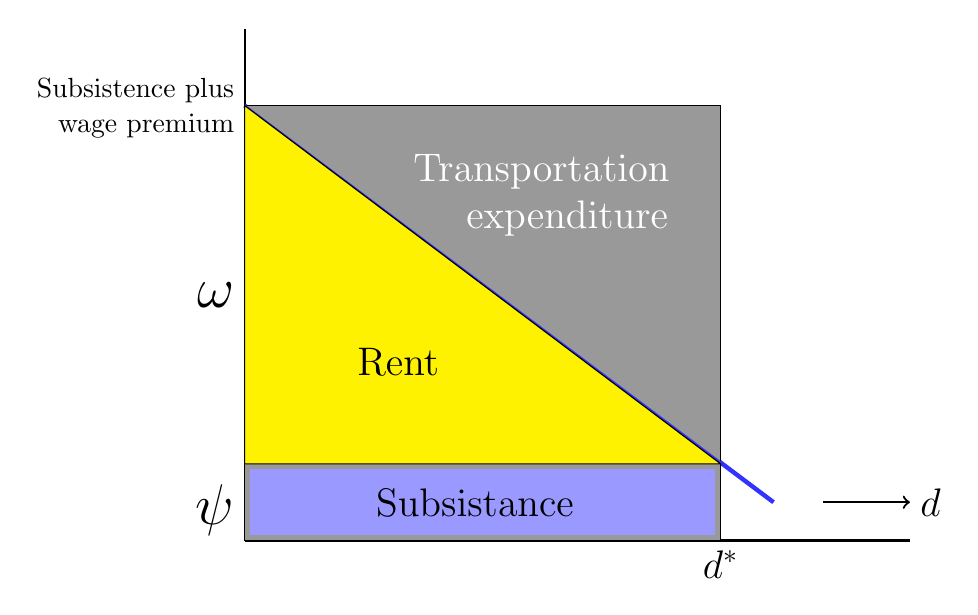
\begin{tikzpicture}[scale=.65]
\def\bndmax{5}        %https://tex.stackexchange.com/questions/68462/filling-a-complex-region-with-tikz
\def\bndmin{0.2}
\def \n {8.5}  % height of y axis
\def \d {13}  % length  of x axis
\def \t {.75}  %  cost of transportation per unit x
\def \th {1}   %
\def \w {7}    %  wage premium
\def \om{1.5}%  omega =rural wage Zero for urban population
\def \azero{2}
\def \aprime {-.0}	
\tikzset{func/.style={thick,color=blue!80}}	

% FIRST FIGURE just axes PARTITIONING THE LABOUR SHARE
\draw [thick] (0,-\om) --(\d,-\om);  			% Zero for rural population
\draw [thick] (0,-\om) --(0,\n); %node[above]{\Huge $w$};	% Y axis
%\node at (0,\n+0.5){\large $Rent$};

% \draw [thick] (0,0)node[left=.5]{Subsistence}--(\d,0);
%\node at(-2,1) {$\omega$};
\node[left=.25] at (0,3.3){\huge $\omega$};
\node[left=.25] at (0,-0.9){\huge $\psi$};
%\node[left=.25] at (0,3){$w+\omega$};
\node[left=.25] at (0,\w+.3){Subsistence plus};
\node[left=.25] at (0,\w-.4){wage premium};	

%\foreach \xi in {0,..., \n} \draw (\xi,0)--(\xi,-.1)node[below=1]{\small$\xi$};
%\foreach \yi in {1,...,\n} \draw (0,\yi)--(-.1,\yi)node[left]{$\yi$};
%\foreach \i in {1,4,9,16} {
%\node at (7,-\om/2){people scattered uniformly across the land  };

%SECOND FIGURE WITH AGGLOMERATION WAGE
%   \pause %  add urban production and net wage PARTITIONING THE LABOUR SHARE
%\draw[fill=white, white] (0.1,-0.1) rectangle (14,-\om+.1);
%\draw [fill=green!80] (-.25, 0) rectangle(.25, \w);
\node[right] at  (.25, \w/2){Added Productivity};
% \node[right, text width = 3cm] at  (10,9){Where does the increase in productivity come from?};
\draw [ thick, ->](11.3,-\om/2)--(13, -\om/2)node [right] {\Large $d$};

%  THIRD FIGURE  add wage profile PARTITIONING THE LABOUR SHARE
% \pause
%\node[right, white, fill=white,  text width = 3cm] at  (10,9){Where does the increase in productivity come from?};
\draw[func, domain=0:\w/\t+1,ultra thick] plot [samples=200] (\x,{\w-\t*\x}); %Net wageprofile  for 
%\node[right, white, fill=white] at  (.25, \w/2){Added Productivity};
%\node[right, fill=white, text width =3.5cm ] at  (1, \w/2){Declining wage  net \\of transportation\\ costs $T(d)$ };

%   FOURTH FIGURE     commuters PARTITIONING THE LABOUR SHARE
%\pause
%\draw[fill=blue!40] (0.1,-0.1) rectangle (9.2,-\om+.1);
%\node at (4.5,-\om/2){commuters};

%   FOURTH FIGURE    wage bill
%\pause %add total new value
\draw[fill=green!40] (0,-\om) rectangle(9.30,\w);% new product
\node at (4.5,\w/2){\Large urban wage bill};

%%   FIFTH FIGURE   distribution
%\pause
%\node at (9,\n){\Large Partitioning the Labour Share};

\draw[fill=black!40] (0,-\om) rectangle (9.30,\w);% new product repeat
\draw[func, domain=0:\w/\t+1] plot [samples=200] (\x,{\w-\t*\x}); %rent profile
\fill[blue!40] (0.1,-0.1) rectangle (9.2,-\om+.1);
\node at (4.5,-\om/2){\Large Subsistance};
\draw[fill=yellow,] (0.,0.) -- (0,7)--(9.30,0.)--cycle;% Rent \w-.2
\node at (3.,2){\Large Rent}; 		%Rent 
\node at (5.8,5.7)[white]{\Large Transportation};
\node at (6.3,4.8)[white]{\Large expenditure};
\node at (9.3,-1.5)[below]{\Large  $d^*$};
% \node at (4.8,\w)[above]{\huge $d^*$};
 \end{tikzpicture}
 

    \caption{ADD CAPTION}
    \label{fig-alonzo-simple}
    \end{center}
\end{figure}

The entire rectangle, $\omega$ $\times$ $d^*$, is the wage bill generated by urban agglomeration. Urban land rent is the residual when transport costs are deducted from the wage premium. It declines  with distance $d$ until, at the very edge of the city, $d^*$, the cost of transportation  consumes the entire wage ($td^*=\omega$). The grey triangle represents the amount of the surplus dissipated in travel costs.  Property values are simply the the present discounted value of the rent at any point.

At the bottom of the figure we illustrate the conventional `subsistence wage'  earned by a worker whether in the city or outside of the city. In most analyses of urban spaces this living wage is simply ignored, since it is the wage premium that generates rents.  The relative size is unimportant because it is the same for urban and non-urban workers. If urban consumption is higher than non-urban consumption it must come out of the land rent.
% Workers are attracted to the city by the wage premium, $\omega$,  which represents the share of the surplus generated by the city that goes to labour.  
\footnote{MOVE TO FUTURE WORK/MENTION AMENITY APPENDIX? If the city generates additional social amenities\index{amenities} not captured in the wage  the money available for housing does not change, although willingness to pay must be higher. The most likely adjustments are in urban `subsistence' and it is probably offset by rural amenity that is given up to live in the city. In the long run urban amenities must exert upward pressure on rural amenities.} % These interesting extension will not be taken up in this thesis.}

The extent  of the city  $d^*$ is a simply the distance at which total $rt$ transportation cost  is equal to the wage premium
\[d^* t= \omega\]
where $t$ is the unit cost of transportation. In the figure, $-t$ is the slope of the diagonal line dividing rent from transportation expenditure.

 \subsection{The magnitude of rents and transportation costs}
 From $w$, $t$ and population density we can derive population, wage bill, total rent, transportation costs. The figure above suggest that  half of the urban surplus is spent on transportation, but because the city is circular, the total value of rents can be represented as  a cone with the volume  \[ V=\frac{1}{3}\pi  d^{*2} \omega \]
of a cone with radius $d^*$ and  height $\omega = td^*$. Substituting out either  $\omega$ or  $d^*$, we find that total rent is  proportional to the \textbf{cube} of either  $d^*$ or $\omega$. 

The total value of wage payments appears as the volume of cylinder enclosing the cone, since the wage is the same for each unit of labour no matter where it resides: 
$V=\pi r^2 \omega$ 
and total transport costs are 
$\frac{2}{3}\pi  d^{*2} \omega).$
With uniform density, population is proportional to the square of  $d^{*2}$ while rents and  transportation costs are proportional to the cube. %move this?

BID-RENT MEANS


\begin{figure}
    \begin{center}
    
\begin{tikzpicture}[scale=.5]
   %%%%%%%%%%%%%%%%%%%%%%%%%%%%%%%%%%%%%%%%%%%%%%%%
% definitions for schematic
\def\bndmax{5}        %https://tex.stackexchange.com/questions/68462/filling-a-complex-region-with-tikz
\def\bndmin{0.2}
\def \n {10}  % height of y axis
\def \d {12}  % length  of x axis
\def \t {.75}  %  cost of transportation per unit x
\def \th {1}   % theta?
\def \w {7}    %  wage premium
\def \om{1.5}%  omega =rural wage Zero for urban population
\def \azero{2}
\def \aprime {-.0}	
\tikzset{func/.style={thick,color=blue!90}}	

    %%%%%%%%%%%%%%%%%%%%%%%%%%%%%%%%%%%%%%%%%%%%%%%%
% definitions for Cone3
%\node at (0, 2.5){\input{SA_Cone3.tex}};
     \pgfmathsetmacro{\radiush}{9.7};%Cone base radius was 9.6
        \pgfmathsetmacro{\theight}{7.1}%Cone height (negative if you want a inverse cone)
        \pgfmathsetmacro{\cheightp}{.03}%Cut height in percent of cone height

        %Calculating coordinates
        \coordinate (center) at (0,0);
        \pgfmathsetmacro{\radiusv}{.2 * \radiush}; %HORIZONTAL RADIUS
        \coordinate (peak) at ($(center) + (0,\theight)$);     
        \pgfmathsetmacro{\sradiush}{\radiush * (1 - \cheightp)};%ADJUST FOR COVERAGE AT CORNERS
        \pgfmathsetmacro{\sradiusv}{.2 * \sradiush};
   %     \pgfmathsetmacro{\sradiusv} {\sradiusv -.1 };

\coordinate (antipeak) at ($(center) + (0,-\theight)$);  %thanks  %I added this
\coordinate (vert1) at ($(center)+(\radiush,-.2)$);
\coordinate (vert2) at ($(center)-(\radiush,.2)$);
%problem
   
\coordinate (svert1) at ($(vert1)!\cheightp!(peak) +(0.1,.75)$);
\coordinate (svert2) at ($(vert2)!\cheightp!(peak)+(.5,.75)$);  
    % \coordinate (svert3) at ($svert1+(0,\w)$);
    % \coordinate (svert4) at ($vert2)+(0,\w)$);  
    %  \coordinate (svert3) at ($svert1+(0,7)$ );  % Shifting up by W
    % \coordinate (svert4) at ($svert2 + (0,\w)$0;
   %%%%%%%%%%%%%%%%%%%%%%%%%%%%%%%%%%%%%%%%%%%%%%%%


 
%\draw[step=.5,black,thin] (-9.6,0) grid (9.6,7);
 
% Cone Drawing    
 \fill[ left color=red!70, right color=red!70,  opacity=20,middle color=red!20,shading=axis] (svert1) -- (peak) -- (svert2) arc (170:370:\sradiush cm and \sradiusv cm);

    % FAT GREEN BAR
 \draw [fill=green,opacity=80] (-.2, 0) rectangle(.2, \w);
 \node[above] at (0,\w){$\omega$};
 
%Uncomment this for top of cylinder
      \fill[inner color=gray!2,outer color=gray!40,shading=radial,opacity=.5] ($(center) + (.35,\theight)$ ) circle (9.4 cm and 1.55 cm );
      
        % \draw [thick]($(svert1) +(.3,-.3)$)-- ++ (90:\w-.2);
        % \draw [thick]($(svert2)-(.2,.3)$)-- ++ (90:\w-.2);
        %Lines, \h in percent of cone height
 def \sradiusv2 \sradiusv cm -.1 cm)
% Cylinder drawing
  \fill[ left color=black!50, right color=red!30,  middle color=red!30,shading=axis,opacity=.2]  (-9.05,.5) 
  arc (180:360:\sradiush cm and \sradiusv cm)-- ++(90:\w-.2) 
  arc (360:180:\sradiush cm and \sradiusv2 cm -.1 cm)--(-9.05,.5);  

   \node[above] at (0,\w){\Large $\omega$};
% TRY TO Make a cylinder
%\draw ($svert2 + (0,\theight)$) [arc (180:360:\sradiush cm and \sradiusv cm)]; 
%     \fill[left color=gray!70,right color=gray!70,middle color=gray!30,shading=axis] (vert1) -- (svert1) arc (0:-180:\sradiush cm and \sradiusv cm) -- (vert2) arc (180:360:\radiush cm and \radiusv cm);

% DASHED LINE AT BACK OF CONE
\foreach \h in {0.03}{   %.38,.34,.30, .7
            \pgfmathsetmacro{\rh}{-\radiush * (1 - \h)}
            \pgfmathsetmacro{\rv}{.2 * \rh}
            \draw[black!70,densely dashed] ($(svert2)!\h!(peak)-(.3,.9)$) arc (370:170:\rh cm and \rv cm);%$(vert2)!\h!(peak)$)
        }
  %      \draw[opacity=.90, line width=.05cm, green] (0,0)--(0,{\theight - .05});
%     \foreach \h in {0, .38,.34,.30, .7}{
%            \pgfmathsetmacro{\rh}{\radiush * (1 - \h)} %            \pgfmathsetmacro{\rv}{.2 * \rh}
%            \draw[black!70,densely dashed] ($(antipeak)!\h!(vert2)$) arc (180:360:\rh cm and \rv cm);
%   }
%  \draw[red] (antipeak) arc (30:60:3);
%  \draw[dashed, thick] arc (0:-180:\sradiush cm and \sradiusv cm) -- (vert2) arc (180:360:\radiush cm and \radiusv cm);
%%%%%%%%%%%%%%%%%%%%%%%%%%%%%%%%%

% %\foreach \xi in {0,..., \n} \draw (\xi,0)--(\xi,-.1)node[below=1]{\small$\xi$};
% %\foreach \yi in {1,...,\n} \draw (0,\yi)--(-.1,\yi)node[left]{$\yi$};
% %\foreach \i in {1,4,9,16} {
% %\node at (7,-\om/2){people scattered uniformly across the land  };

% %SECOND FIGURE WITH AGGLOMERATION WAGE
% %  add urban production and net wage
% %\draw[fill=white, white] (0.1,-0.1) rectangle (14,-\om+.1);

% \node[right, text width=4cm] at  (3, \w+1){Added Productivity due to agglomeration};
% %\node[right, text width = 3cm] at  (10,9){Where does the increase in productivity come from?};
 \draw [ thick, ->](0,0)--(2.5, 0)node [right] {\Large $d$};


% \draw[thick] (0,0) -- ++ (50:2.6cm);  %   diagonal for perspective
% \draw[thick] (0,0) -- ++ (230:2.35cm); 

% %  THIRD FIGURE  add RENT profile in blue

% %\node[right, white, fill=white,  text width = 3cm] at  (10,9){Where does the increase in productivity come from?};
% \draw[func, domain=0:\w/\t+1,ultra thick] plot [samples=200] (\x,{\w-\t*\x}); %Net wageprofile  for 
% %\node[right, white, fill=white] at  (.25, \w/2){Added Productivity};
% %\node[right, fill=white, text width =3.5cm ] at  (1, \w/2){Declining wage  net \\of transportation\\ costs $T(d)$ };
% %\node[right, fill=white, text width =3.5cm ] at  (4,9){Declining wage  net \\of transportation\\ costs  };
% %
% %\node at (0, 1.5){\includegraphics{\input{SA_Cone3.tex}} };
% %\node at (0, 2.5){\input{SA_Cone3.tex}};

% %   FOURTH FIGURE     commuters
% %\pause
% %\draw[fill=blue!40] (0.1,-0.1) rectangle (9.2,-\om+.1);
% \node at (4.5,.4*\om){commuters};


\end{tikzpicture}
    \caption{Wage bill, transportation costs and rent as a residual.}
    \label{fig-city-conical}
    \end{center}
\end{figure}


%%%%%%%%%%%%%%%%%%%%%%%% PARTITIONING THE LABOUR SHARE
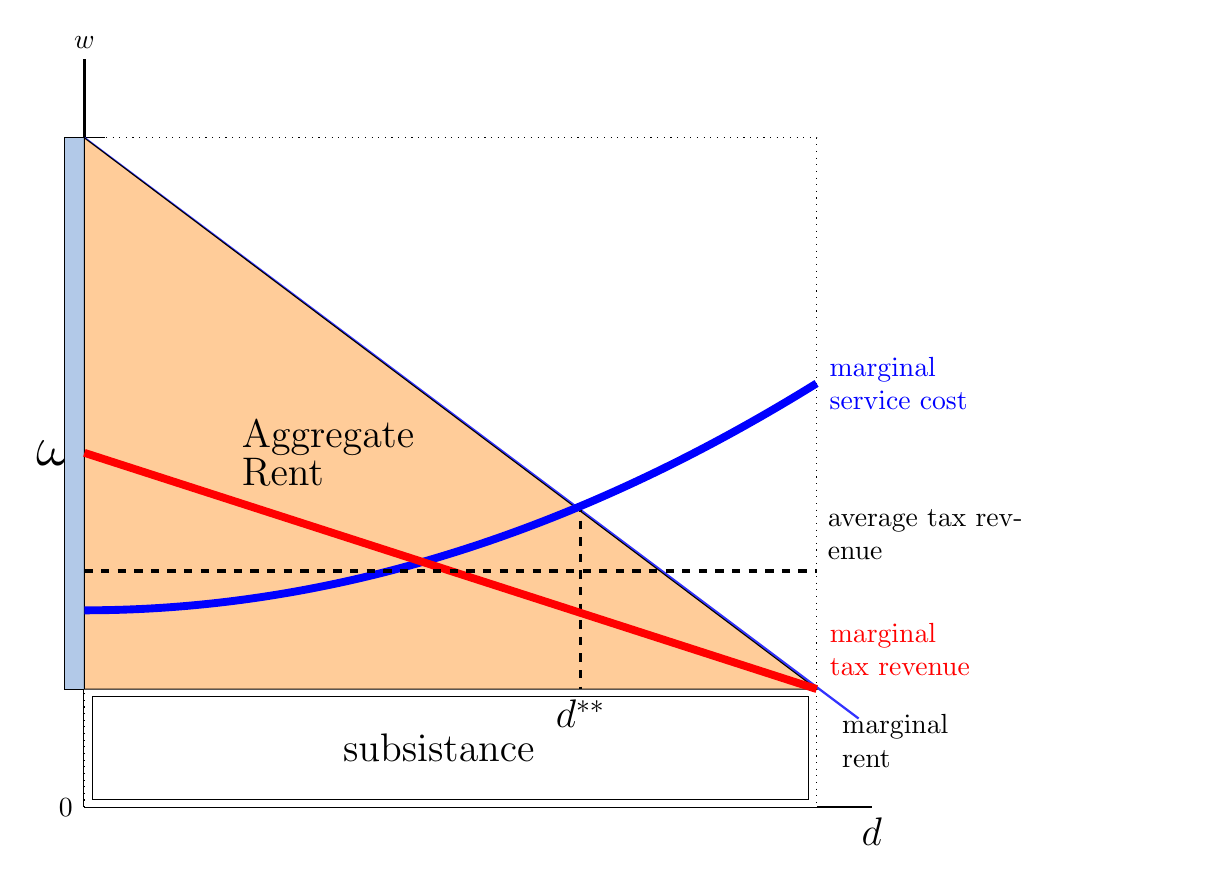
\begin{tikzpicture}[scale=1]
\def\bndmax{5}        %https://tex.stackexchange.com/questions/68462/filling-a-complex-region-with-tikz
\def\bndmin{0.2}
\def \n {8}  % height of y axis
\def \d {10}  % length  of x axis
\def \t {.75}  %  cost of transportation per unit x
\def \th {1}   %
\def \w {7}    %  wage premium
\def \om{1.5}%  omega =rural wage Zero for urban population
\def \azero{2}
\def \aprime {-.0}	
\tikzset{func/.style={thick,color=blue!80}}	
\draw [thick] (0,-\om) --(\d,-\om)node[below]{\Large$d$};  			% Zero for rural population
\draw [thick] (0,-\om)node[left=.5]{$0$} --(0,\n)node[above]{$w$};	% Y axis

%\draw [thick] (0,0)node[left=.5]{ subsistance}--(\d,0);
\node[left=.25] at (0,3){\huge $\omega$};
%\node[left=.25] at (0,\w+.3){subsistence plus};
%\node[left=.25] at (0,\w-.4){wage premium};	

\draw[fill=white, white] (0.1,-0.1) rectangle (14,-\om+.1);
\draw [fill=green!30!blue!30] (-.25, 0) rectangle(.25, \w);
\node[right] at  (.25, \w/2){Added Productivity};
%\draw [ thick, ->](11.3,-\om/2)--(13, -\om/2)node [right] {\Large $d$};
\draw[fill=blue!40] (0.1,-0.1) rectangle (9.2,-\om+.1);

\draw[fill=black!0, dotted] (0,-\om) rectangle (9.30,\w);% new product repeat
\draw[func, domain=0:\w/\t+.5] plot [samples=200] (\x,{\w-\t*\x}); %rent profile
\draw[fill=blue!0] (0.1,-0.1) rectangle (9.2,-\om+.1);
\node at (4.5,-\om/2){\Large subsistance};
\draw[fill=orange!40,] (0.,0.) -- (0,7)--(9.30,0.)--cycle;% Rent \w-.2
\node[text width=2cm] at (3.,3){\Large Aggregate \\Rent}; 		%Rent 
%\node at (5.8,5.7)[]{\Large Transportation};
\node at (6.3,4.8)[white]{\Large expenditure};
\draw[ line width=.5mm, dashed] (6.3,2.35)--(6.3,0)node[below ]{\Large$d^{**}$};

\draw[func, domain=0:9.3, line width=1mm,blue, text width=2cm] plot [samples=200] (\x,{1+\x^2/30})node[right]{marginal\\ service cost};
\draw[ line width=1mm, red] (0,3)--(9.3,0)node[above right, text width=3cm ]{marginal\\tax revenue};
\node at (9.5, -.2)[below right, text width=2cm]{marginal rent};

\draw[ line width=.5mm, dashed] (0,1.5)--(9.3,1.5)node[above right, text width=2.5cm ]{average tax revenue};

%GRID
%\draw[step=1cm,gray,very thin] (0,0) grid (10,10);

 \end{tikzpicture}
 
% \section{Other work developing the urban model}
% ADD -DEFINITION OF bid-rent, 
\section{Development of the urban model}
What we refer to the basic model as the Alonzo model, but was developed by several scholars in parallel in roughly the same period. 
% We will refer to the core urban model developed by 
It was developed by 
Alonso \cite{alonsoLocationLandUse1964}, Muth \cite{muthCitiesHousingSpatial1969} and Mills \cite{millsAggregativeModelResource1967}, and later formalised by Wheaton \cite{wheatonComparativeStaticAnalysis1974} and others, as the ``Alonzo Model.''\footnote{it is also called the Alonzo model, the Alonzo-Muth model, the Alonzo-Muth-Mills model, the circular city model, and the monocentric city model.} William Alonso published \textbf{Location and Land Use} in 1964  \cite{alonsoLocationLandUse1964} based on his 1960 Phd thesis,\cite{alonsoModelUrbanLand1960} 
giving him a slender priority in the literature.  (***E ADD ... % He was concerned with.... His model did.... INTRODUCE THE WORK ITSELF)

Richard Muth's \cite{muthSpatialStructureHousing1961}, and \cite{muthRationalExpectationsTheory1961}  were written roughly simultaneously with and independently of Alonso's thesis, and  culminated in Muth's classic book, Cities and Housing  \cite{muthCitiesHousingSpatial1969}.\footnote{See ``William Alonzo, Richard Muth, Resources for  the Future, and the founding of urban economics''\cite{mcdonaldWilliamAlonsoRichard2007} for a more detailed discussion of the development of the model.}  % ***E ADD % This workoverlps with Alonzo in these ways. Differed in these ways... USE THIS TO FLESH OUT MORE OF THWAT HIS MODEL?WORK ISDOING AND HOW

It is worth noting that Lowdon Wingo also had what appears to be a working paper, ``Transportation and Urban Land'' \cite{wingoTransportationUrbanLand1961}, for the organization Resources for the Future  in preparation for publication that presented a core idea and  significantly influenced Muth \cite{mcdonaldWilliamAlonsoRichard2007}. Mills' ``Urban economics'' \cite{millsUrbanEconomics1972} followed soon after. The early 1960s were a watershed in urban economics, and the model rapidly became the workhorse for theorists and empirical researchers.

EXPLAIN BID RENT CURVE
 The seeds of the \gls{bid-rent curve} at the heart of the model were presented as early as 1885  by German engineer-economist Wilhelm Launhardt. \cite{blaugEconomicTheoryRetrospect1985, launhardtMathematischeBegruendungVolkswirthschaftslehre1885} The  \gls{bid-rent function} was first applied explicitly to the equilibrium of land use patterns in agricultural production by August Losch \cite{loschEconomicsLocation1954} in Germany and Edgar S. Dunn \cite{dunnEquilibriumLandUsePatterns1954} in America, and was later extended to the urban setting by William Alonso \cite{alonsoModelUrbanLand1960}. 
 
\subsection{Limitations of the basic model}
% Net land rent} 
The simple graphical model we consider above is revealing, but it leaves out many important features of the urban system. The only costs included are the transportation costs for the individual.  Since urban services and  a substantial fraction of urban amenities are financed through the public sector a more complete model must include both servicing costs and property taxation. The relevant rent profile from an economic point of view is net of all service costs. From a financial point of view, it is net of tax liabilities.% It would be interesting to produce a 3-D graph of the NET rents. 

...

\section{Extensions on the urban model}

The urban model is a basic model and there have been many extensions FIGURE
% Figure showing variations and modern adaptations of the model.


The Alonzo model, long  recognized as a persistent ``law'' in urban and regional studies, 
is actually a model of competitive real estate markets: in less than competitive markets, other factors may affect bid-rents significantly.

Gao et al.\cite{GaoJinlong2020BtbT}, for example,  found  that for China, ``other exogenous  factors –– including the distinct land system  and centralized political institutions -- also matter a great deal''. In general, however, 
research has largely supported the bid-rent model (\cite{mutoEstimationBidRent2006, wheatonBidRentApproach1977}) Muto \cite{mutoEstimationBidRent2006}, for example concluded that,  ``land usage on average follows the rule that is consistent with the bid-rent function model: whichever usage outbids the others occupies the land. ''  Borba1 and Dentinhoand \cite{borbaEvaluationUrbanScenarios2016} concluded that ``The method has proved its usefulness and effectiveness for predicting the impacts of exogenous shocks in complex urban systems.'' 
%
In a test for the city of Bogota, Gross \cite{grossEstimatingWillingnessPay1988} found that  ``the bid-rent model works reasonably well in its predictions and in its estimates of the demand for attributes and, in some ways, it may perform better than a hedonic-type model in forecasting the demand for housing attributes.'' 

Clay and Valdez incorporate bid-rent model into an integrated ABM transportation-land use mode that achieves levels of accuracy similar to the best models currently available. These are the microsimulation of UrbanSim;\footnote{UrbanSim is a microsimulation land use model, designed to support the need of Metropolitan Planning Organizations (MPOs), cities and other organizations for analyzing the potential effects of land use policies and infrastructure investments on the development and character of cities and regions. The core model code has been developed in the Python programming language as Open Source software and is publicly available on the Urban Data Science Toolkit GitHub page.\cite{waddellmodellinurbandev2002}} and the bid-rent sub-module of \footnote{PECAS is  HBA Specto Incorporated's commercial modelling system  for simulating spatial economic systems.} developed by Abraham and Hunt (2005). the best models currently available. They emphasises the advantage of ABM model is allowing for agents to differ in composition and in preferences making them unique bidders. 
% Agents must compute the maximum bid price they are willing to pay.
An earlier analysis by Curran and Carlson \cite{curranTheoryResidentialLocation1982}, among other, extended the bid-rent model include two-worker households and a secondary employment location. They showed that households would be expected to segregate spatially, but the pattern will depend on the specific combination of wages, transport costs and the mix of household types in the populations. 

\section{Implications of Alonzo's urban model}
Even with all its simplifications, the model  can  describe  many features of urban structure and urban history. In this section, we illustrate some of the insights supported by the model. Extensions can incorporate variations in wages, density, transportation costs,  preference, and even building technology and codes. The limitations of the simple, continuous, equilibrium-based versions described above can be overcome using agent-based models to model the evolution of complex and much more realistic urban systems. 

For example, two stylized facts should be noticed. The first is that the marginal cost of servicing generally  rises with the distance from the centre.  ADD Figure
%~\ref{}
illustrates the general form of servicing costs, but not  the relative scales of rent and servicing costs. When this observation is combined with the `Henry George Theorem" () the conclusion is that the optimal size of the city  is at  $d^{**}$, where marginal service cost intersects with the marginal increase in total urban rent. 

The second stylized fact is that property taxes, which are generally  fixed as a share of property value, decline as the distance from the centre increases. Figure %~\ref{} 
illustrates the general form of tax liabilities, although it does not  accurately represent their relationship to rent or  servicing costs.  This implies that in many or most urban situations the residents at the outer edges pay less than the average amount in property tax per unit of land, but cost  the community budget more than the average amount. In essence, the central city subsidizes the suburbs. (ref Perverse Cities)
This arrangement is both economically inefficient and unfair, but it has been built into the fiscal structure of cities largely as a result of automobile-based urban growth. It is likely that this fiscal misallocation saps some of the potential productivity growth of cities.

Property taxation reduces the market value of properties, but it also funds services and amenities that increase the value of properties. 

Both servicing and taxation effects are more variable and than the simple model suggests.  One conclusion urban theorists draw based on variants of the Alonzo model is that because property owners in the low-density urban margin are subsidized,  the subsidy is likely to create serious fiscal problems for municipalities in the long-term and result in serious inefficiency in land use.

\section{Summary}
In this chapter we have described % a very abstract, 
stylized models, establishing how the urban system generates rents. % and relating them to neoclassical growth theory.  
In the next chapter, we'll link the basic spatial model to the scaling of urban productivity, by modelling the agglomeration effects.

This chapter introduces the background to the theory of the urban model. This is important because we will essentially build that standard urban model into our model of financialization and in the process we will be adding to the standard urban model the distributional consequences that have been over looked, by carrying the concept of rent through to explore the distributional consequences and how the distribution of rents feeds back into the productivity of cities. 

Our base model builds on this basic classic urban Alonzo model, so it will capture core features with a simple established framework to connect with the existing literature.  
One feature of this model is that none of the simplifying assumptions are essential. We maintain the basic simplicity, but the mode can easily be generalized in many ways, and there is a substantial body of work extending and varying each of the simplifications in the model, as discussed above, as well as substantial work grounding and testing the model empirically.